%%%%%%%%%%%%%%%%%%%%%%%%%%%%%%%%%%%%%%%%%%%%%%%%%%%%%%%%%%%%
%%%  Thesis template for Brown University dissertation format
%%%   http://www.brown.edu/Divisions/Graduate_School/academics/index.php?p=2-11-4&s=2-11
%%%
%%% Modified to fit Brown U by: R. M. Strain
%%% Date: Feb. 2006
%%%
%%%  Thrown together by: Duane Q. Nykamp
%%%  Date: April, 2000
%%%
%%%  Use at your own risk. Not guaranteed to meet 
%%%  requirements. But this is an attempt to make formatting
%%%  a thesis in LaTeX easier.
%%%
%%%  Good luck. Feel free to improve.
%%%
%%%  Large parts apparently lifted from Barry Smith and Mark Asch
%%%%%%%%%%%%%%%%%%%%%%%%%%%%%%%%%%%%%%%%%%%%%%%%%%%%%%%%%%%%



\documentclass[12pt,oneside]{amsbook}
\usepackage{graphicx}

\makeindex

%%%%%%%%%%%%%%%%%%%%%%%%%%%%%%%%%%%%%%%%%%%%%%%%%%%%%%%%%%%%
%%%  Hack for appendices
%%%
%%%  If have single appendix remove the [multiple] option
%%%  from appendixhack, and comment out the
%%%  list of appendices below
%%%%%%%%%%%%%%%%%%%%%%%%%%%%%%%%%%%%%%%%%%%%%%%%%%%%%%%%%%%%

%\usepackage[multiple]{appendixhack}


%%%%%%%%%%%%%%%%%%%%%%%%%%%%%%%%%%%%%%%%%%%%%%%%%%%%%%%%%%%%
%%%  Set title, names, and date
%%%%%%%%%%%%%%%%%%%%%%%%%%%%%%%%%%%%%%%%%%%%%%%%%%%%%%%%%%%%

\newcommand{\thesistitle}{Mathematical Lessons from Peanuts}
\newcommand{\myname}{Charlie Brown}
\newcommand{\degrees}{B.~S., College of Peanuts, 2000\\  Sc.~M., Brown University, 2002}
\newcommand{\advisor}{Snoopy}
\newcommand{\readerone}{Woodstock}
\newcommand{\readertwo}{Pigpen}
\newcommand{\readerthree}{Linus}
\newcommand{\dean}{Marcie}
\newcommand{\department}{Division of Comic Strips}
\newcommand{\thesismonth}{May}
\newcommand{\thesisyear}{2005}


%%%%%%%%%%%%%%%%%%%%%%%%%%%%%%%%%%%%%%%%%%%%%%%%%%%%%%%%%%%%
%%%  Specify depth of table of contents
%%%  0 -- include only chapters
%%%  1 -- include chapters and sections
%%%  2 -- include chapter, sections, and subsections
%%%%%%%%%%%%%%%%%%%%%%%%%%%%%%%%%%%%%%%%%%%%%%%%%%%%%%%%%%%%

\setcounter{tocdepth}{2}


%%%%%%%%%%%%%%%%%%%%%%%%%%%%%%%%%%%%%%%%%%%%%%%%%%%%%%%%%%%%
%%%  Set the Margins
%%%%%%%%%%%%%%%%%%%%%%%%%%%%%%%%%%%%%%%%%%%%%%%%%%%%%%%%%%%%

%\pdfpagewidth=8.5in  	% Width of the PDF page to create (i.e. size of paper you'd print on)
%\pdfpageheight=11in 	% Height of the PDF page to create (i.e. size of paper you'd print on)
\topmargin=0.0in    		% Margin at top of page above all printing
\oddsidemargin=0.5in	% Left margin on odd numbered pages
\evensidemargin=0.5in	% Left margin on even numbered pages
\headheight=0.0in		% Height of the header (the header is text that appears atop all pages
\topskip=0.0in			% Distance from top of main text box to the baseline of the first line of text in the main text box.
\textheight=9.0in		% Height of main text box.
\textwidth=6.0in		% Width of main text box.
%\headsep=0.0in		% Distance from bottom of header to the body of text on a page.
%\footskip=0.0in			% Distance from bottom of body to the bottom of the footer 
%\parskip				% Distance between paragraphs.
%\parindent				% Amount of indentation at the first line of a paragraph.

%%%%%%%%%%%%%%%%%%%%%%%%%%%%%%%%%%%%%%%%%%%%%%%%%%%%%%%%%%%%
%%%  Uncomment to include only specfic sections
%%%%%%%%%%%%%%%%%%%%%%%%%%%%%%%%%%%%%%%%%%%%%%%%%%%%%%%%%%%%

% \includeonly{title,frontispiece,acknowledge,preface,abstract}
% \includeonly{introduction}
% \includeonly{concusion}



\tolerance=400  %allow slightly looser typesetting for fewer
                %overfull boxes


\bibliographystyle{abbrv}

\begin{document}

\linespread{1.6}   %double spaced
\normalsize        %set to normalsize so double spacing kicks in

\pagenumbering{roman}  % front matter number with roman
\pagestyle{plain}

\frontmatter

%%-------------------------------------Title page (unnumbered)
\thispagestyle{empty}


\begin{center}
\huge\bfseries 
\thesistitle
\end{center}
  \vfill
  \begin{center}%
    by\\
\myname \\
    \degrees
  \end{center}
  \vfill
  \begin{center}
    A Dissertation submitted in partial fulfillment of the\\
    requirements for the Degree of Doctor of Philosophy\\
    in the \department~at Brown University
  \end{center}
  \vfill
  \begin{center}
    Providence, Rhode Island\\
    \thesismonth~\thesisyear
  \end{center}
 % include always starts on a new page

%%-------------------------------------Copyright  (unnumbered)
\vspace*{2in} 
\begin{center}
\copyright~Copyright
\thesisyear~by \myname
\end{center}

\thispagestyle{empty} \hbox{   } \newpage

%%-------------------------------------Signature Page




  \begin{center}
    This dissertation by \myname~is accepted in its present form \\
    by the \department~as satisfying the  \\
    dissertation requirement for the degree of Doctor of Philosophy.
  \end{center}



\vfill




\begin{tabular}{lc}
Date \rule{1in}{.05mm}\hspace*{.75in} & \rule{3in}{.05mm}\\
        & \advisor, Director
\end{tabular}

\vfill

  \centerline{Recommended to the Graduate Council}%\\[.75in]
  
   \vspace{.4in}
  
  \begin{tabular}{lc}
Date \rule{1in}{.05mm}\hspace*{.75in} & \rule{3in}{.05mm}\\
        & \readerone, Reader
\end{tabular}\\[.4in]

  \begin{tabular}{lc}
Date \rule{1in}{.05mm}\hspace*{.75in} & \rule{3in}{.05mm}\\
        & \readertwo, Reader
\end{tabular}\\[.4in]

  \begin{tabular}{lc}
Date \rule{1in}{.05mm}\hspace*{.75in} & \rule{3in}{.05mm}\\
        & \readerthree, Reader
\end{tabular}
  
\vfill

  \centerline{Approved by the Graduate Council}

 \vspace{.4in}

  \begin{tabular}{lc}
Date \rule{1in}{.05mm}\hspace*{.75in} & \rule{3in}{.05mm}\\
        & \dean, Dean of the Graduate School
\end{tabular}


%\end{center}



\newpage


%%-------------------------------------Vitae Page
\chapter*{Vit\ae}


The very first Peanuts comic strip appeared on October 2, 1950.  This is also the first time Charlie Brown is called "Good Ol' Charlie Brown." 


\newpage


%%-------------------------------------Frontispiece (optional, unnumbered)

\vspace*{3in} 
\begin{center}
``Good Grief!''
\end{center}


 


%%-------------------------------------Dedication, (first numbered)
\pagestyle{plain}
\vspace*{3in} 
\begin{center}
{\large\em Dedicated to Peppermint Patty}
\end{center}

\addcontentsline{toc}{chapter}{Dedication}
\hbox{   } \newpage

%%-------------------------------------Acknowledgements
\chapter*{Acknowledgements}


I thank Charles Schulz, who else?

\newpage

%%-------------------------------------Preface
\chapter*{Preface}


Writing a dissertation about the mathematics of Peanuts is a difficult
endeavor. I'm glad to have completed it in time to graduate.

\bigskip

\begin{flushright}
\parbox{2in}{\em
\myname\\[2mm]
Providence, Rhode Island
}
\end{flushright}

\newpage

%%-------------------------------------TOC
\tableofcontents

%%-------------------------------------LOT
\listoftables

%%-------------------------------------LOF
\listoffigures

%%-------------------------------------Abstract
%\lipsum[6-8]
            
\newpage




%%-------------------------------------Thesis body
\mainmatter
\pagenumbering{arabic}   %start arabic numbering

\section{Introduction}\label{introduct}
A well-studied phenomenon in material science concerns the coarsening of microstructure found in metals, porcelains, and other common materials.  Typically, these materials have polycrystalline structure, where each grain has a particular orientation.  Annealing induces an evolution on grain boundaries which reduces their total length.  During this process, grains are deleted (and not created), causing coarsening of microstructure through an increase of average grain area (see Fig. \ref{samplegrains}).  Microstructure can determine material properties. For instance, the Hall-Petch effect gives a relation between yield stress and average grain size (see \cite{anderson2005fracture}, section 5.2.3).     More scientific and  mathematical properties of grain networks can be found in \cite{fradkov1994two,thompson2001grain}.


 
 
Grain coarsening in two dimensions  can be modeled by a geometric network, or planar graph $G(t) \subset \mathbb{R}^2$, $t\in (0,T)$, with edges  that evolve in time. Faces of $G$ are called \textbf{grains}, and edges are referred to as \textbf{boundaries}. An idealization of the coarsening process assumes that grain boundaries are isotropic, or that grain boundary energies are identical along edges of the network. Under this idealization, we  define a \textbf{grain network with existence interval} $(0,T)$  as a geometric finite planar graph $G(t)$ which satisfies the
following restrictions for all $t\in(0,T)$:



\begin{enumerate}
\item (\textbf{Herring's Condition})   $G(t)$ is trivalent, and angles between two edges at a vertex are fixed at 120 degrees.
This restriction follows from a force balance law on edges  emanating from a vertex (see \cite{herring1999surface}).\item (\textbf{Mean Curvature Flow}) Boundaries are smooth, and satisfy mean curvature flow.  This means that the time evolution of a smooth boundary $\gamma(x,t)\subset \mathbb R^2$ is also smooth, and satisfies 
 \begin{equation} \label{curveflow}
\partial_t \gamma(x,t) = M\sigma \kappa(x,t)  \vec n(x,t), \quad t\in(0,T), x \in \mathbb{R}^2,
\end{equation}
with $M$ and $\sigma$ denoting grain mobility and surface energy constants, $\vec n(x,t)$ denoting the inward unit normal, and $\kappa(x,t)$ denoting mean curvature. This type of motion was observed experimentally by Beck for crystallites in metals \cite{bec52}.
\end{enumerate}
     


Note that grain networks retain their topological structure during their existence time.  The parabolic PDE (\ref{curveflow})  is referred to as curve-shortening flow, and it can in fact be shown that the total edge length of a network decreases in time \cite{barmak2011entropy}. A theorem of curve shortening flow on grain networks, due to von Neumann and Mullins \cite{mul56,von1952discussion} gives an elegant relation between a topological quantity (sides of a grain) and a geometrical quantity (area of a grain).

\begin{figure}
\includegraphics[width=\textwidth]{samplegrains.png}
\caption{\textbf{Coarsening of a grain network.} Grains in material microstructure delete through annealing, causing the average grain size to increase.}\label{samplegrains}
\end{figure}
 


\begin{theorem}(\textbf{The von Neumann-Mullins $n-6$ rule}). For a grain with area $A$ and $n$ sides,
\begin{equation}
\frac{dA}{dt} = M\sigma\frac \pi 3 (n-6).
\end{equation}  
\end{theorem}
One consequence of the $n-6$ rule  is  that grains with less than six sides may shrink to a point in finite time. Such deletions, along with possible edge deletions, result in networks with vertices that violate Herring's condition.  This raises the question: What types of solutions exist with initial conditions that are not grain networks?  Specifically, the \textbf{continuation problem for a planar network $G$} asks the following: If we are given a planar network $G$ with vertices that may not satisfy Herring's conditions,  is there an  $\varepsilon>0$ where $G(t)$ is a grain network for $t\in (0, \varepsilon)$, and $G(t)\rightarrow G$ in the Hausdorff distance as $t\rightarrow  0^+$? Another interesting question is whether the flow is unique, or if it can become unique under additional assumptions.

Currently, there are no comprehensive answers to the above questions.  Viewed as a problem in parabolic PDE theory, the current focus is local, fixing on simplified models with initial conditions of $k$ rays meeting at a vertex. Schnurer and Shulze found a unique self-similar solution with initial conditions of three rays meeting at arbitrary angles \cite{sch07}.  Mazzeo and Saez  generalized with the $k$-ray initial conditions, and discovered a bijection between self-similar solutions   and $k$-Steiner trees of a hyperbolic metric \cite{maz07}.  On the computational front, techniques of flowing through a graph not satisfying the grain network conditions include level set \cite{elsey2009diffusion}  and variational \cite{kin06} methods. 
 




\section{Mean-field models of grain growth}\label{fradkov}
Another approach to studying grain boundary coarsening involves using mean field assumptions to gather bulk statistics of grain behavior.  A well known kinetic model is due to Fradkov \cite{fra882,fra881}, who exploits  the $n-6$ rule, along with an additional deterministic rule for side redistribution, to derive kinetic equations for densities of grains with a specific number of sides.   Fradkov makes the following mean field assumptions about the redistribution of sides when either a grain or edge deletes:
\begin{enumerate}
\item If a grain or side deletes, topological changes of grains will be selected in proportion to the number of sides of grains, and independent of their areas.  For instance, if a singular event causes a grain to lose a side, the probability that a particular grain with $j$ sides will drop to one with $j-1$ sides is
\begin{equation}
p_j=\frac{j}{\sum_{k>1} kN_k},
\end{equation}
where $N_k$ is the number of grains with $k$ sides.  
  This eliminates the notion of grains having neighbors.  
\item A free parameter $\beta$ is introduced which is defined as the constant ratio between side deletions and grain deletions.  Such an assumption comes from the lack of a topological rule for edge growth.  
\end{enumerate}

For a number density $f_n(a,t)$ of $n $ sided grains with area $a$ at time $t$, the Fradkov equations take the form of a transport equation with a topological source term:
\begin{equation}
\partial_t f_n(a,t)+(n-6)\partial_a f_n(a,t) = \Gamma(f(t))(Jf)_n(a,t) \quad (a,t) \in (0,\infty)^2, n \ge 2 ,
\end{equation}
with a collision operator $J$ and coupling weight $\Gamma$ determined from conservation of area and polyhedral defect (networks retain an average of six sides). Well-posedness and self-similar solutions for the Fradkov model can be found in \cite{henseler2008kinetic, her12}.



 
\section{PDMPs and grain coarsening}\label{pdmpgraincoarse}
The main goal of this thesis is to understand grain  statistics as a hydrodynamic limit of finitely many grains respecting deterministic drift and random topological transitions.  In particular, we will  construct limiting kinetic equations describing the evolution of grain area densities for the class of grains with a fixed number of sides.   Toward this goal, the main tool we use is the theory of piecewise deterministic Markov process (PDMP).  The construction and theory of PDMPs will be discussed in Chapter 2.  However, not much is lost to think of a PDMP  as a generalization of a jump process for particles that drift on vector fields.    

For the problem of grain coarsening, we wish to build a PDMP $X(t)$ that tracks a finite set of grains $(g_1,\dots, g_n) =  ((a_1,s_1), \dots, (a_n,s_n))$ with areas $a_i>0$ and side numbers $s_i \in \mathbb N.$  
Note that the dimension of $X(t)$ can change with time, as grains delete from coarsening. Grain areas change at a constant rate, following the $n-6$ rule until a grain shrinks to a point, or an edge deletes (we will make an assumption on side deletion rates based on total particle number).  At that time, we impose mean field assumptions to change topologies of grains. 

 

 
\begin{figure}  
\begin{centering} 
 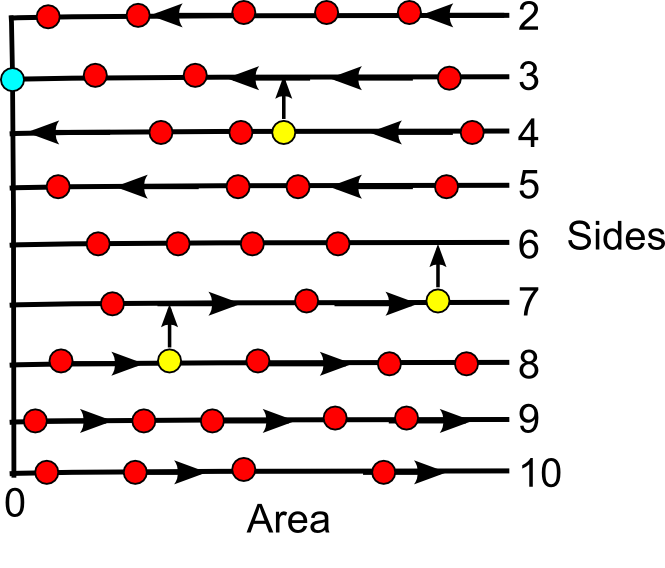
\includegraphics[width = .4\textwidth]{graintops.png} 
 \caption{\textbf{Grain growth via a PDMP}. Particles drift according to their number of sides. Each tier denotes particles of different side numbers. In this instance, a vanishing grain in tier three triggers a  random reassignment  of the number of sides of grains in tiers 4,7, and 8.}
\end{centering}
\end{figure}

\section{Overview}
 
In Chapter 2, we describe a PDMP in generality. We then state its infinitesimal generator $\mathcal A$, and the class of functionals $\mathcal D(\mathcal A)$ that give rise to martingales through the Dynkin formula.    

In Chapter 3, we  study a simplified version of the PDMP described in Section \ref{pdmpgraincoarse}. Here, particles drift on the positive half-line until reaching the origin, where they are reassigned according to a probability density $p(x)$.     We first prove that for empirical densities approaching nonatomic initial conditions, the densities $u(x,t)$ of particles converge to a weak form of the limiting kinetic equation
\begin{alignat}{2}\label{pde1}  
\partial_tu(x,t) - \partial_x u(x,t) = p(x)u(0,t) \quad t, x \in \mathbb{R}^+, \\
u(x,0) = u_0(x) . \nonumber
\end{alignat}
We then focus on constructing measure valued weak solutions of (\ref{pde1}) with mild restrictions on initial data. Finally, we use a popular result of renewal theory to show the existence of an attractor under certain assumptions.

  Chapter 4 is a generalization of PDMPs on grain networks described in Section \ref{pdmpgraincoarse}.  Here, we show the existence of fluid limits of PDMPs that allow generalized rules and probability distributions for particle jumps between different species.  As in Chapter 3, we will show the existence of a weak limit for densities $u_k(x,t)$ on $L_k$, that satisfy the advection-reaction equations
\begin{eqnarray} \label{pde2}
  \lefteqn{\partial_t u_k(x,t)+\partial_{x}(v_k(x)u_{k}(x,t))=  \phantom{u_j(x,t)\mathbf{1}_{R^{(l)}_{ij}}
-K^{(l)}W_k^{(l)}(t)u_k(x,t)}}\label{smoooth}\\
 && \sum_{l = 1}^{M_-}u_l(0,t)v_{l}(0)\left[\sum_{i = 1}^{M}\sum_{j= 1}^{K^{(l)}} W_i^{(l)}(t)u_i(x,t)\mathbf{1}_{R^{(l)}_{ij}=k}
-K^{(l)}W_k^{(l)}(t)u_k(x,t)\right]\nonumber\\ 
&&+\frac{\beta G(t)}{G^{int}(t)}\left( \sum_{i = 1}^{M}\sum_{j= 1}^{K^{int}} w^{int} _iu_{i}(x,t)\mathbf{1}_{R^{int}_{ij} = k}-K^{int}w^{int}_ku_{k}(x,t)
 \right), \nonumber
 \end{eqnarray}
 with initial conditions
 \begin{equation}
u_k(x,0) = u_{k}^0(x), \quad k = 1,\dots, M. \nonumber
\end{equation}
The solutions of (\ref{pde2}) will be shown to be unique in the class of $L^1\cap L^\infty(\mathbb R^+)$ functions.

Finally, in Chapter 5, we return to the problem of grain coarsening. First, we examine the topological behavior of grain networks before and after a grain or side vanishes. After finding a finite set of rules that dictate topological changes,    we then define the various free parameters in the $k$-species model to align with a mean field model for grain coarsening.  Next, we prove some basic properties of the limiting kinetic equation, such as conservation of mass and polyhedral defect.  Finally, we end the chapter with a computational investigation of grain growth, and raise several conjectures about grain statistics.   
  

 

\chapter{Meet the Peanuts}\label{FAQ}



\section{Who are they?}

Snoopy\index{Snoopy} is an extroverted beagle with a Walter Mitty complex. He is a virtuoso at every endeavor- at least in his daydreams atop his doghouse. He regards his master, Charlie Brown, as ``that round-headed kid'' who brings him his supper dish. He is fearless though prudently cautious about ``the cat next door.'' He never speaks- that would be one human trait too many- but he manages to convey everything necessary in facial expressions and thought balloons. A one-man show with superior intelligence and vivid imagination, he has created such multiple personalities as: Joe Cool, World War I Flying Ace, Literary Ace, Flashbeagle, Vulture, Foreign Legionnaire, etc.


Charlie Brown wins your heart with his losing ways. It always rains on his parade, his baseball game, and his life. He's an inveterate worrier who frets over trifles (but who's to say they're trifles?). Although he is concerned with the true meaning of life, his friends sometimes call him ``blockhead.'' Other than his knack for putting himself down, there are few sharp edges of wit in his repertoire; usually he's the butt of the joke, not the joker. He can be spotted a mile away in his sweater with the zig zag trim, head down, hands in pocket, headed for Lucy's psychiatric booth. He is considerate, friendly and polite and we love him knowing that he'll never win a baseball game or the heart of the little red-haired girl, kick the football Lucy is holding or fly a kite successfully. His friends call him ``wishy-washy,'' but his spirit will never give up in his quest to triumph over adversity.

Woodstock is the smallest of the Peanuts characters but has a big presence for a little bird. He's a little inept, his flying and logic are erratic, but he can type and take shorthand and usually is game for anything Snoopy\index{Snoopy} wants to do. Although he's the butt of many of Snoopy\index{Snoopy}'s practical jokes, he's the beagle's closest friend and confidant- and has made attempts at retaliation. Because of his size and the company he keeps, Woodstock is an accident waiting to happen. Being a bird and tiny, he gets a little insecure around Thanksgiving and big moving objects. He's the only baseball player who gets an automatic walk if the ball rolls over him. Woodstock talks birdspeak only, and finds an alphabet made up entirely of exclamation points quite adequate to express such emotions as distress, frustration and a real temper. His flocking friends are Bill, Harriet, Olivier and Conrad.

Linus Van Pelt inspired the term ``security blanket'' with his classic pose. He is the intellectual of the gang, and flabbergasts his friends with his philosophical revelations and solutions to problems. He suffers abuse from his big sister, Lucy, and the unwanted attentions of Charlie Brown's little sister, Sally. He is a paradox: despite his age, he can put life into perspective while sucking his thumb. He knows the true meaning of Christmas while continuing to believe in the Great Pumpkin.


Lucy Van Pelt works hard at being bossy, crabby and selfish. She is loud and yells a lot. Her smiles and motives are rarely pure. She's a know-it-all who dispenses advice whether you want it or not--and for Charlie Brown, there's a charge. She's a fussbudget, in the true sense of the word. She's a real grouch, with only one or two soft spots, and both of them may be Schroeder, who prefers Beethoven. As she sees it, hers is the only way. The absence of logic in her arguments holds a kind of shining lunacy. When it comes to compliments, Lucy only likes receiving them. If she's paying one--or even smiling--she's probably up to something devious.


Sally Brown's brother, Charlie Brown, was so pleased and proud when she was born that he passed out chocolate cigars. Since then he's been trying to understand her. She always looks for the easy way out, particularly at school, where her view of life reflects much of the frustration and confusion kids experience. Her speech is riddled with malapropisms. Uninhibited, and precocious, she has a schoolgirl crush on Linus, her ``Sweet Babboo.'' She may never win Linus' heart, but she has her big brother wrapped around her little finger. Sally, writing letters or doing homework, causes pain and joy to her fans in roughly equal proportions.



Schroeder, who idolizes Beethoven, brought classical music to the Peanuts strip. Reserved and usually unruffled, Schroeder reacts only when Woodstock tries to make his grand piano into a playground, or Lucy seeks to make it her courting grounds. The latter can lead to minor violence.



Peppermint Patty is a pro on the baseball diamond, but in the classroom she's a D-minus all the way. Bold, brash and tomboyish, what she lacks in common sense she makes up for in sincerity. She's the only one who calls Charlie Brown ``Chuck.'' Oblivious to much that goes on around her, for a long time she seemed unaware that ``the funny-looking kid who plays shortstop'' was a beagle. She has trouble staying awake in class; most of her waking hours in the schoolroom are spent analyzing the probability patterns of true-false tests.


Marcie\index{Marcie} is Peppermint Patty's best friend. From the moment they met at summer camp, Marcie\index{Marcie} has called Peppermint Patty "Sir" out of admiration and misguided manners. An unlikely pair, they seem to have nothing in common yet that is what makes their friendship so genuine. Marcie\index{Marcie} is the smartest of the Peanuts gang, but also the most naive. She's always willing to help out her friend with school work and she's not above sharing test answers or calling her on the phone to remind her of homework assignments. There is an innocence to Marcie\index{Marcie} and Peppermint Patty is her protector. Marcie\index{Marcie} is also completely inept when it comes to sports, yet they still let her play on the baseball team. If Marcie\index{Marcie} and Peppermint Patty ever have a falling out it's likely to be over Charlie Brown, who they both secretly love.


Before grunge was cool, Pigpen\index{Pigpen} made his debut in the Peanuts comic strip on July 13, 1954 and since then has been the butt of "dirt" gags. He walks around in a cloud of dust, sprinkling dirt on all he comes in contact with. Pigpen\index{Pigpen} is happily messy. He doesn't try to explain it, hide it, fight it. For him, it's just a fact of life. His slovenly ways paid off in 1993 with a series of television commercials for Regina vacuum cleaners which combined animation with live-action.


Franklin met Charlie Brown at the beach in 1968. They'd never met before because they went to different schools, but they had fun playing ball so Charlie Brown invited Franklin to visit him at this house across town for another play session. Later, Franklin turned up as center-fielder on Peppermint Patty's baseball team and sits in front of her at school. Franklin is thoughtful and can quote the Old Testament as effectively as Linus. In contrast with the other characters, Franklin has the fewest anxieties and obsessions. He and Charlie Brown spend quite a bit of time talking about their respective grandfathers. When Franklin first appeared in the late 60s, his noticeably darker skin set some readers in search of a political meaning. However, the remarkable becomes unremarkable when readers learn that Schulz simply introduced Franklin as another character, not a political statement.


Rerun Van Pelt is often mistaken for Linus even though he's his little brother. He can always be recognized in his trademark overalls. Rerun is more skeptical than his brother, much harder to convince, and always gets around Lucy where Linus gives in. His only fear is being the passenger on one of his mother's bicycle-riding errands. Somehow, Rerun is the only witness to her riding into grates and potholes. Luckily, he always wears a helmet. Rerun also longs for a dog of his own, but since his parent won't let him have one, he tries to ``borrow'' Snoopy\index{Snoopy} from Charlie Brown. Snoopy\index{Snoopy} won't have any part of it unless Rerun brings cookies.



\section{Furthermore}

Peanuts was one of the first comic strips with more than two or three characters. Just like your own family and relatives, each Peanuts character brings special humor and insight to life.\footnote{Everything in this chapter was ungraciously reproduced from {\em http://www.unitedmedia.com/} to check formatting.  This is not at all intended for reproduction.}


\chapter{Conclusion}


\section{Future extensions}

\subsection{Garfield}

\begin{figure}
\centering

\includegraphics[width=1in]{garfield.pdf}
\caption{Garfield}
\end{figure}


\subsection{The Far Side}


\section{Alternative Perspectives}

Different, less mathematical perspectives on Peanuts have been
written. \cite{peanutsgospel}



%%-------------------------------------Appendix or Appendices

\appendix

\chapter{Parameters}


An appendix.

\chapter{Other stuff}

Another appendix.
 % input is the same as include, but it doesn't need to start on a new page



%%----------------------------BIBLIOGRAPHY
\backmatter
\newpage

%\addcontentsline{toc}{chapter}{Bibliography}

\bibliography{thesis}

\renewcommand{\indexname}{(Incomplete) Index of Peanuts}
\printindex

\end{document}

